\documentclass[reprint,amsmath,amssymb,aps,prb,nofootinbib]{revtex4-2}

\usepackage{graphicx}% Include figure files
\usepackage{dcolumn}% Align table columns on decimal point
\usepackage{bm}% bold math
\usepackage{xcolor}
\usepackage{listings} % insert code fragments
\usepackage{braket}
\usepackage{quantikz}
\usepackage{hyperref}% add hypertext capabilities

\definecolor{codegreen}{rgb}{0,0.6,0}
\definecolor{codegray}{rgb}{0.5,0.5,0.5}
\definecolor{codepurple}{rgb}{0.58,0,0.82}
\definecolor{backcolour}{rgb}{0.95,0.95,0.92}

\lstdefinestyle{mystyle}{
    backgroundcolor=\color{backcolour},   
    commentstyle=\color{codegreen},
    keywordstyle=\color{magenta},
    numberstyle=\tiny\color{codegray},
    stringstyle=\color{codepurple},
    basicstyle=\ttfamily\footnotesize,
    breakatwhitespace=false,         
    breaklines=true,                 
    captionpos=b,                    
    keepspaces=true,                 
    numbers=left,                    
    numbersep=5pt,                  
    showspaces=false,                
    showstringspaces=false,
    showtabs=false,                  
    tabsize=2
}

\bibliographystyle{plainnat}

\lstset{style=mystyle}

\begin{document}
    \title{Entanglement Heating, Entanglement Cooling \& Irreversibility}
    \author{Hendrik Kühne}
    \affiliation{Technical University of Munich}
    \date{\today}

    \begin{abstract}
        We show that irreversibility emerges from microscopically reversible dynamics in the entanglement
        and subsequent disentanglement of quantum states. To this end, we entangle an initial random quantum state
        using gates chosen randomly from a set of gates, and try to disentangle it with a Metropolis-inspired
        algorithm. The emergent dynamics do not depend on the particular choice of the set of gates, but only
        on whether the chosen gate set is universal or not. Furthermore, we show that the spacing of consecutive
        singular values reveals if the disentanglement procedure succeeds or not: Universal gate sets induce spacings
        that follow the Gaussian Orthonormal Ensemble spacings, while non-universal gate sets induce Poisson-like
        distributed spacings. This is an example of Loschmidt's
        Paradox in quantum systems, revealing the universal tension between microscopically reversible dynamics
        and macroscopic irreversibility.
    \end{abstract}

    \maketitle

    \section{Introduction}

    How can irreversible phenomena in phyiscs occur? This question has been unanswered for a long time
    \cite{Loschmidt:1876:LoschmidtParadox}, and has been treated from different angles
    \cite{Haar:1955:FoundationsStatisticalMechanics,Shaffer:2014:IrreversibilityAndEntanglement}. The heart of
    the problem is that the microscopical laws of nature (Classical Mechanics, Particle Physics) are reversible
    in nature, yet macroscopic dynamics can be irreversible, as is set in stone most famously by the second law
    of thermodynamics.

    Recently, this question has been approached using Quantum Mechanics and, more specifically, entanglement
    \cite{Shaffer:2014:IrreversibilityAndEntanglement,Odavic:2023:RandomUnitaries,Chamon:2014:EmergentIrreversibility}.
    The question of irreversibility seems even less tractable in Quantum Mechanics; all dynamics are unitary and
    thus reversible. Non-unitary dynamics occur only when considering, e.g. quantum channels, which model unitary
    dynamics from the perspective of a subsystem. Subsystems experience the non-classical phenomenon of entanglement
    among each other, making this a natural entry point for irreversibility to be introduced into Quantum Mechanics.

    In this work, we show how the creation of entanglement is irreversible in the sense that random dynamics cannot,
    under certain conditions, disentangle the systems under consideration. The paper is structured as follows: We introduce
    the formalism of entanglement and the algorithm in Section~\ref{sec:theory}. Afterwards, we give details on
    the simulations we carried out in Section~\ref{sec:simulation}. Our results are discussed in Section~\ref{sec:results}.

    \section{Entanglement and Universality}
    \label{sec:theory}

    Quantum Mechanics offers many phenomena that are thoroughly non-classical, most notably entanglement. The term
    ``entanglement'' refers to a phenomenon where the state of one system cannot be fully described without knowledge
    of another system; we say that the two systems are ``entangled''. Consider the Hilbert space $\mathcal{H}$,
    and states $\rho$ therein. The full Hilbert space may be partitioned into two spaces
    $\mathcal{H}=\mathcal{H}_A\otimes\mathcal{H}_B$. The state on subsystem $A$ then becomes

    \begin{equation}
        \rho\mapsto\text{tr}_B\rho\equiv \rho_A.
        \label{theory:eq:reduced_state}
    \end{equation}

    If there exist states $\ket{\psi_A}\in\mathcal{H}_A$ and $\ket{\psi_B}\in\mathcal{H}_B$ s.t.
    $\rho=\ket{\psi_A}\bra{\psi_A}\otimes\ket{\psi_B}\bra{\psi_B}$, we say $\rho$ is a product
    state. If, on the other hand, we can write

    \begin{equation}
        \rho=\sum p^{(i)}\rho_A^{(i)}\otimes\rho_B^{(i)},
        \label{theory:eq:separable_state}
    \end{equation}

    we call $\rho$ a ``separable state''. In both cases, there is no entanglement present in the system, since we are
    able to express the state using objects that live in only one of the subsystems. If on the other
    hand, $\rho$ is not a product state, i.e. there are no $\rho_A^{(i)}$, $\rho_B^{(i)}$ s.t. Equation~\ref{theory:eq:separable_state}
    holds, then we say $\rho$ is ``entangled''. This means that $\rho$ cannot be fully characterized from the two
    subsystems; it lives on the bipartite Hilbert space.

    Entanglement sits at the core of many non-classical effects of Quantum Mechanics \cite{Einstein:1935:EPR} and
    is used widely in Quantum Computing \cite{Harrow:2009:hhlAlgorithm,Shor:1997:PolyTimeFactorizing}, making it
    not only a mechanism of high conceptual relevance but also a resource to be used in computation.

    Entanglement can be measured by the von-Neumann entanglement entropy $S$. Consider again the ``reduced state''
    $\rho_A$ on subsystem $A$, that results from tracing out subsystem $B$ (Equation~\ref{theory:eq:reduced_state}).
    Diagonalizing $\rho_A$ gives it's spectrum $\sigma=\{\lambda_i\}$ of eigenvalues. The entanglement entropy of
    this state is defined as\footnote{Note that we have introduced entanglement as a notion that is only explainable
    by considering bipartite systems, yet we are defining a measure of entanglement using an object that lives on
    only one of the systems. This is possible because the spectrum $\sigma$ of the reduced state $\rho_A=\text{tr}_B\rho$
    is related to the Schmidt coefficients of the state on the whole system. Let $\sigma=\{\lambda_i\}$ and let
    $\rho=\ket{\psi}\bra{\psi}$ be a pure state. Then it's Schmidt decomposition is
    $\ket{\psi}=\sum_i\sqrt{\lambda_i}\ket{\psi_A^{(i)}}\otimes\ket{\psi_B^{(i)}}$. This explains why it is possible to
    characterize the entanglement between two subsystems by considering the reduced state on one of the systems.}

    \begin{equation}
        S(\rho_A) = -\text{tr}\left(\rho_A\log_2\rho_A\right) = -\sum_i\lambda_i\log_2\lambda_i.
    \end{equation}

    Non-entangled states give $S(\rho)=0$, while $S(\rho)>0$ signifies the presence of entanglement. In particular,
    $S(\rho)=0$ for separable states and product states.

    \vspace{\baselineskip}

    Let us now consider states of $N$ qubits, such that the Hilbert space is $\mathcal{H}=\mathbb{C}^{2^N}$. The state of this system may be changed by applying unitary transformations
    $U:\mathbb{C}^{2^N}\rightarrow\mathbb{C}^{2^N}$. We refer to these as ``gates'', in analogy to classical
    computing. Gates may act on an arbitrary number of qubits. Gates that act on more than one qubit can create
    entanglement, while single-qubit gates do not change the entanglement that is present in the system.
    The irreversibility-paradox in Quantum Mechanics comes to be since transformations $U$ of quantum states are
    unitary, and thus reversible. Since entanglement can be created, it can thus also be destroyed.

    \vspace{\baselineskip}

    In this work we investigate the possibility of entanglement being created and then destroyed by
    random quantum circuits. The first step consists of creating entanglement. Starting from a random product state

    \begin{equation}
        \ket{\psi}=\ket{\psi}_0\otimes...\otimes\ket{\psi}_{N-1},
    \end{equation}

    we iteratively and randomly choose a gate $U$ from a set $\mathcal{I}$ and apply it to a random subset of
    qubits. Single-qubit gates further randomize the state, while multi-qubit gates create entanglement. The
    entanglement creation is measured by the von-Neumann entropy $S(\rho_A)$: For every iteration, we measure
    the entanglement entropy $S_{N_A}$ for every bipartition

    \begin{equation}
        \mathbb{C}^{2^N}\mapsto\mathbb{C}^{2^{N-N_A}}\otimes\mathbb{C}^{2^{N_A}}
        \label{theory:eq:bipartition}
    \end{equation}

    into two systems of $N_A$ and $N-N_A$ (consecutive) qubits, respectively. This iterative procedure creates a random quantum state, which we can
    expect to be highly entangled with high probability \cite{Page:1993:AverageEntropy,Hamma:2012:RandomQuantumEntanglement}.
    After entanglement has been created, we try to disentangle the state using a Metropolis-inpired algorithm
    \cite{Shaffer:2014:IrreversibilityAndEntanglement,Odavic:2023:RandomUnitaries,Chamon:2014:EmergentIrreversibility}:
    In every iteration, we choose again a random gate $U\in\mathcal{I}$ from the same set of gates, and apply it to
    a random set of qubits. In doing this we obtain the new state $\ket{\psi^{(j+1)}}=U\ket{\psi^{(j)}}$. We measure
    the entanglement and obtain, after the $j$th iteration, the entanglement entropies $\{S_{N_A}^{(j)}\}$ of
    every bipartition (recall Equation~\ref{theory:eq:bipartition}). Some gates will increase $S$, while others
    decrease it. The new state $\ket{\psi^{(j+1)}}$ is accepted if the mean entanglement entropy $\braket{S_{N_A}^{(j+1)}}\equiv S^{(j+1)}$
    has decreased\footnote{To be more specific, $\braket{S_{N_A}^{(j+1)}}=\frac{1}{N-1}\sum_{N_A=1}^{N-1}S_{N_A}^{(j+1)}$,
    i.e. we are averaging over the bipartitions of Equation~\ref{theory:eq:bipartition}.}. If entanglement has not
    decreased, we accept it with a probability

    \begin{equation}
        P = e^{-\beta(S^{(j+1)}-S^{(j)})},
        \label{theory:eq:metropolis_update}
    \end{equation}

    where $\beta$ plays the role of an inverse temperature. Emphasizing the similarity to the Metropolis algorithm
    \cite{Metropolis:1953:EquationsOfState}, we call this second step ``entanglement cooling''. Conversely,
    the first step is referred to as ``entanglement heating''.

    \section{Heating and Cooling simulations}
    \label{sec:simulation}

    In this section, we give details on the numerical simulation of the heating and cooling steps.
    In both steps, we simulate quantum states $\ket{\psi}$ as full statevectors $\ket{\psi}\in\mathbb{C}^{2^N}$.

    \vspace{\baselineskip}

    \subsection{Entanglement heating}
    \label{sec:simulation:heating}

    As per convention in Quantum Computing, the initial state is $\ket{0}^{\otimes N}$.
    A random product state is created by applying the rotation gate

    \begin{equation}
        R_Y(\theta) = e^{-i\theta Y/2} \doteq \left(\begin{array}{cc}
            \cos(\theta/2) & -\sin(\theta/2) \\ \sin(\theta/2) & \cos(\theta/2)
        \end{array}\right)
    \end{equation}

    on every qubit, with angles $\theta$ randomly selected from $[0,\pi]$. Afterwards, we choose randomly a gate
    $U$ from a gate set $\mathcal{I}$ and choose randomly the qubits it is applied to. The gate sets we investigate
    are

    \begin{equation}
        \begin{array}{cc}
            \{\text{CNOT},H,Z\}, & \{\text{iSWAP},H,T\}, \\
            \{\text{CNOT},H,X\}, & \{\text{iSWAP},H,S\}, \\
            \{\text{CNOT},H,S\}, & \{\text{iSWAP},H,X\}, \\
            \{\text{CNOT},H,T\}, & \{\text{iSWAP},H,Z\}.
        \end{array}
    \end{equation}

    Note that among these, only $\{\text{CNOT},H,T\}$ and $\{\text{iSWAP},H,T\}$ are universal gate sets
    \cite{Forest:2015:CliffordUniversality} (see also Figure~\ref{simulation:fig:iSWAP}). A universal
    gate set is a gate set such that every unitary operation can be approximated with arbitrary precision using
    gates from the set.

    \begin{figure}
        \begin{quantikz}
            \qw & \swap[partial swap={i},label style={scale=2}]{1} & \midstick[2,brackets=none]{=} & \gate{S} & \gate{H} & \ctrl{1} & \targ{}   & \qw      \\
            \qw & \targX{}                   &                               & \gate{S} & \qw      & \targ{}  & \ctrl{-1} & \gate{H}
        \end{quantikz}
        \caption{The $\text{iSWAP}$ gate is reducible to $H$, $S$ and $\text{CNOT}$ using the circuit identity above. Recall also
        that $S=T^2$, so the universality of $\{\text{iSWAP},H,T\}$ follows from the universality of $\{\text{CNOT},H,T\}$.}
        \label{simulation:fig:iSWAP}
    \end{figure}

    We apply $R_{\text{heat}}=250$ gates during the heating procedure. This gives a highly entangled state $\ket{\psi_{\text{heat}}}$.

    \subsection{Entanglement cooling}
    \label{sec:simulation:cooling}

    The entanglement cooling step starts with the state $\ket{\psi_{\text{heat}}}$ that the heating step terminated in. On this
    state, we again apply a random gate $U\in\mathcal{I}$ from the gate set that was used in the heating step,
    again on a random set of qubits. The new state is only accepted if the mean entanglement decreases, or with
    the probability given in Equation~\ref{theory:eq:metropolis_update}. This is repeated for $R_{\text{cool}}=6000$
    iterations, with $\beta$ fixed.

    \vspace{\baselineskip}

    We repeat heating and cooling $100$ times and average over the results. The number $N$ of qubits was chosen as
    $N\in [4,11]$ and the (inverse) temperature is $\beta=5$, if not stated otherwise.

    \section{Results}
    \label{sec:results}

    The heating rate is consistent across different realizations, with negligible deviations. The entanglement of states with different
    sizes $N$ grows with the same rate, before individual system sizes converge to their maximum entanglement. An
    explanation for the comparable rates of entanglement creation is rooted in the fact that we are using two-qubit gates
    to create entanglement. A two-qubit gate can only create entanglement between the two qubits it is applied to, and
    the entanglement in such a system is limited to $S\leq\log_2d=2$. Thus, no matter the system size, the gates we use
    create entanglement at the same rate.

    The maximum entanglement we reach during the heating step is proportional to $N$:

    \begin{equation}
        \max_{N_A}\braket{S_{N_A}} \propto N.
    \end{equation}

    This is in line with the known scaling $S\propto \log_2d$ \cite{Page:1993:AverageEntropy} of the entropy of a random
    quantum state, where $d$ is the dimension of the local Hilbert space (recall that here, $d=2^{N_A}$). The rate of entanglement
    creation is slightly smaller for gate sets that contain the $\text{iSWAP}$ gate, but maximum entanglement values are
    equal. See also Figure~\ref{results:fig:therm_examples}.

    \vspace{\baselineskip}

    The entanglement cooling rate does not depend on the value of $\beta$; for $\beta\in [1,10]$, cooling occurs at the
    same rate. See Figure~\ref{results:fig:betatest}.

    \begin{figure}[htb]
        \includegraphics[width=\columnwidth]{plots/betatest_{CNOT,H,X}_CNOT.pdf}
        \caption{We simulated entanglement cooling for $\beta\in [1,10]$ in a system of four qubits ($N=4$) and the gate
        sets $\{\text{CNOT},H,X\}$, $\{\text{CNOT},H,S\}$ and $\{\text{CNOT},H,T\}$. There is no difference in the cooling
        rate, as is shown above for one particular gate set.}
        \label{results:fig:betatest}
    \end{figure}

    We move on to the central result of this work, which concerns irreversibility: The entanglement cooling step
    does not always succeed. If the creation of entanglement were reversible, cooling would always be able to lower
    the entanglement back (or close to) zero\footnote{Where disentangling succeeds, there remain differences in how
    much entanglement the cooling step is able to remove from the state. The gate sets that contain $\text{CNOT}$ are
    able to fully disentangle the state in question. The sets containing $\text{iSWAP}$ are able to remove a
    significant amount of entanglement, however, they cannot reduce $S$ back to zero. See
    Figure~\ref{results:fig:therm_CNOT_vs_iSWAP}.}; this is not the case, however. Specifically, entanglement cooling fails,
    whenever the gate set that is used is universal. Disentangling occurs at the same rate regardless of system
    size $N$ and whether it succeeds or fails, for the same reason that entanglement heating occurs at the same
    rate\footnote{Stated more precisely, the shapes of the curves of $\braket{S_{N_A}}$ match. The process of disentangling
    starts later for larger systems, however. Why this is remains an intriguing direction for future work.}.
    Disentangling begins later during the cooling process for larger systems. See also Figure~\ref{results:fig:therm_spped_iSWAP}.

    \begin{figure}[htb]
        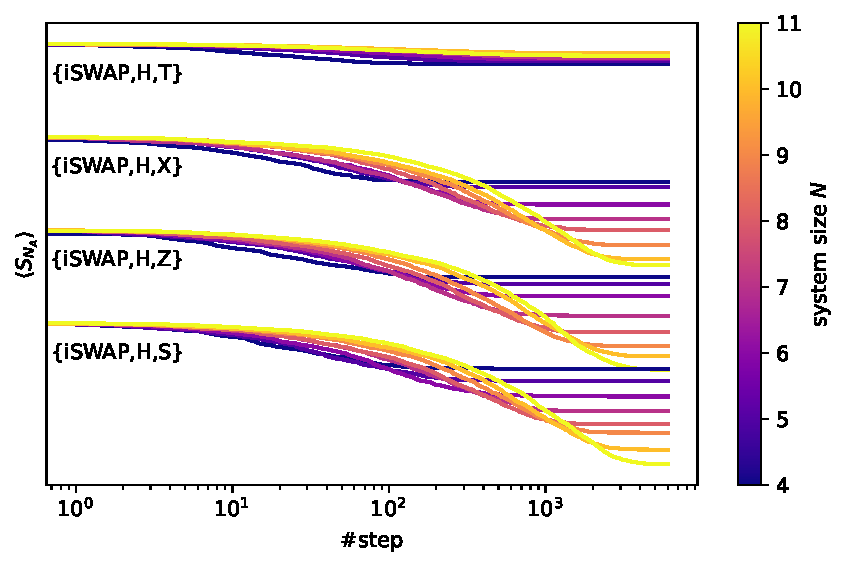
\includegraphics[width=\columnwidth]{plots/therm_speed_iSWAP.pdf}
        \caption{The entanglement cooling process for gate sets that contain an $\text{iSWAP}$ gate. This plot only shows differences
        in mean entanglement. The rate of disentangling is similar for different gate sets.}
        \label{results:fig:therm_spped_iSWAP}
    \end{figure}

    At this point we may ask ourselves how we can characterize the scenarios where disentangling succeeds, versus the
    ones where it does not. The answer can be found in the spectrum of consecutive spacings of Schmidt values. Consider
    the equal bipartition of a system of size $N$ in two parts of size $N_A = \lfloor N/2\rfloor$ and $N_B=N-N_A$. The
    spectrum of the associated density matrices $\rho_A$ and $\rho_B$ is $\sigma_{N/2}=\{\lambda_i\}$, and it coincides
    with the Schmidt values of the complete state $\ket{\psi}$. Assume the Schmidt coefficients $\lambda_i$ to be sorted
    in descending order, then the consecutive spacings are $\Delta_i = \lambda_i-\lambda_{i+1}$. Their expected distribution

    \begin{equation}
        P(\Delta\lambda) = \sum_{i=0}^{N-2}\braket{\delta(\Delta-\Delta_i)}
        \label{results:eq:spacing_distribution}
    \end{equation}

    differs for states that were generated using different gate sets. States that stem from universal gate sets show
    spacing statistics that closely follow the Gaussian Orthogonal Ensemble (GOE) \cite{Chamon:2014:EmergentIrreversibility}.
    This refers to the distribution of eigenvalue spacings of random orthogonal matrices \cite{Mehta:2003:RandomMatrices};
    the ``Wigner surmise'' states that their distribution can be described by \cite{Guler:2007:RandomMatrixTheoryIntrodution}

    \begin{equation}
        P(\Delta) \approx C\Delta^{\beta}e^{-A\Delta^2},
        \label{results:eq:wigner_surmise}
    \end{equation}

    for appropriately chosen $C$, $\beta$, $A$. The spacing statistics of states from non-universal gate sets exhibit
    a different distribution, more closely related to a Poisson-distribution. This holds true for gate sets containing
    either $\text{iSWAP}$ or $\text{CNOT}$. See Figure~\ref{results:fig:level_spacing_head_CNOT}.

    \begin{figure}[htb]
        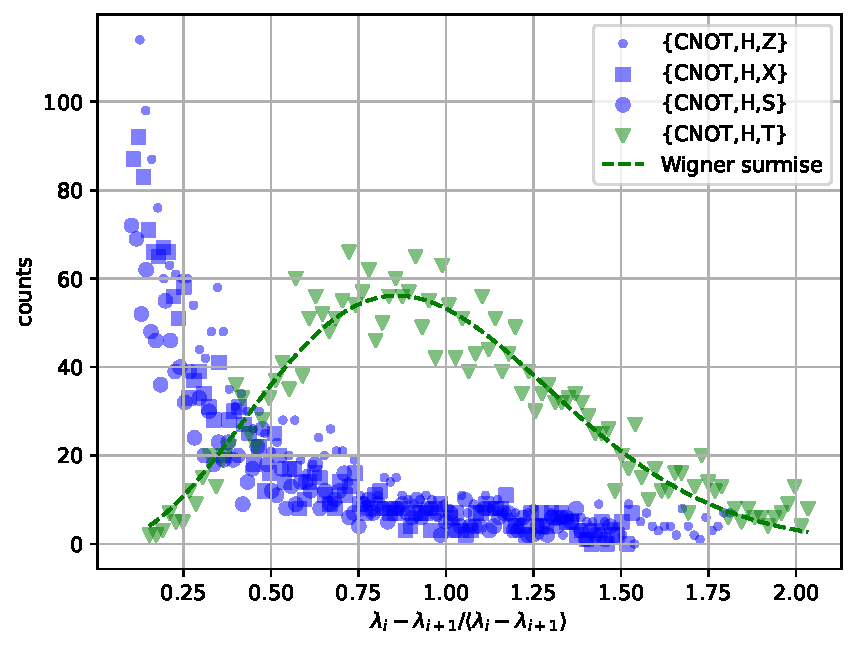
\includegraphics[width=\columnwidth]{plots/level_spacing_head_CNOT.pdf}
        \caption{The level spacing statistics of states with $N=11$, that were generated with gate sets that contain
        the $\text{CNOT}$ gate. While the universal set $\{\text{CNOT},H,T\}$ procuces states whose spacings follow the
        GOE very closely (Equation~\ref{results:eq:wigner_surmise}), the non-universal sets follows a Poisson-like
        distribution. The same holds true for gate sets that contain the $\text{iSWAP}$ gate. This plot only shows
        values $\Delta/\braket{\Delta}$ below a value of $2$, since the distributions have a long tail. The interested
        reader is referred to Ref.~\cite{Kuehne:2024:EntanglementCooling}, where all distributions are shown.}
        \label{results:fig:level_spacing_head_CNOT}
    \end{figure}

    \section{Conclusion \& Outlook}
    \label{sec:outlook}

    Our results demonstrate that the conflict between microscopically reversible dynamics and macroscop irreversibility
    can be modelled with and found in Quantum Mechanics, specifically in the entanglement of chains of qubits. We demonstrated
    that randomly generated circuits of single- and two-qubits gates consistently generate highly entangled states at the
    same rate. Disentangling these states with a Metropolis-inspired algorithm only succeeds when the gate set used to
    generate the state in question is not universal. The ability of a state to be disentangled is encoded in the distribution
    of consecutive Schmidt coefficient spacings. For states that can be disentangled, these follow a Poisson-like
    distribution. The spacings of states that cannot be disentangled follow the GOE distribution. This enables us to
    treat Loschmidt's Paradox with the tools of Quantum Mechanics and Quantum Computing, thereby opening up avenues for
    further investigation of the topic.

    \vspace{\baselineskip}

    The value in the method we presented lies in the fact that we are not limited to using statistical methods, as is
    the case in thermodynamics and statistical physics. Our system of $N$ qubits has a comparably small amount of degrees
    of freedom, and it's interaction with the environment we subject it to (i.e. the gates we apply) are very well understood
    and can be easily and exactly simulable. Yet, even in such a controlled environment, we find irreversibility emerging
    from reversible dynamics.

    \vspace{\baselineskip}

    There remain open questions. Consider for example the aforementioned result that $\text{iSWAP}$-sets create entanglement
    at a rate slighly slower than $\text{CNOT}$-sets, and the fact that non-universal $\text{iSWAP}$-sets are unable to
    remove all entanglement from the system. A more exact characterization of the rates at which entanglement
    is created remains a topic for future work; specifically, if entanglement heating and cooling rates can be increased
    or decreased depending on the set of gates that is used. A further open question concerns the observation that the
    disentangling process starts later for larger systems, but progresses at the same rate once it has begun.

    A further question that deserves more attention stems from wondering whether a $\text{CNOT}$-set can disentangle a state
    that was created using an $\text{iSWAP}$-set, and vice-versa. Since the spacing statistics of $\text{CNOT}$-states
    and $\text{iSWAP}$-states agree, one could expect the answer to be yes; then again, $\text{iSWAP}$-containing sets
    cannot completely disentangle a state, but only partially. Put more broadly: In what capacity is the ability to be
    disentangled a property of a quantum state, or of the gate set that is used?

    \bibliography{references}

    \begin{figure*}[htb]
        \includegraphics[width=\columnwidth]{plots/therm_{CNOT,H,Z}.pdf}
        \includegraphics[width=\columnwidth]{plots/therm_{iSWAP,H,T}.pdf}
        \caption{Two examples of the thermalization of entanglement, i.e. the heating and cooling steps, for two
        different gate sets. The rates of entanglement heating are very similar, with the $\text{iSWAP}$ gate creating
        entanglement slighly slower than the $\text{CNOT}$. The maximum entanglement that is reached scales linearly with
        system size $N$. Cooling succeeds for the non-universal gate set $\{\text{CNOT},H,Z\}$, it fails however for the
        universal $\{\text{iSWAP},H,T\}$.}
        \label{results:fig:therm_examples}
    \end{figure*}

    \begin{figure*}[htb]
        \includegraphics[width=\columnwidth]{plots/therm_{CNOT,H,Z}.pdf}
        \includegraphics[width=\columnwidth]{plots/therm_{iSWAP,H,Z}.pdf}
        \caption{Two examples of the thermalization of entanglement, i.e. the heating and cooling steps, for two
        gate sets that only differ in which two-qubit gate they contain. The $\text{CNOT}$-containing set is able
        to remove all entanglement from the state, while disentangling converges at a value $S\neq 0$ for
        $\text{iSWAP}$-containing gate sets. Notice that the reamining entanglement scales linearly with the system
        size, just as the maximum entanglement does.}
        \label{results:fig:therm_CNOT_vs_iSWAP}
    \end{figure*}

    \appendix

    \section{Code Availability}

    The code to carry out the simulations as well as the data can be found in the corresponding GitHub Repository
    \cite{Kuehne:2024:EntanglementCooling}.

\end{document}
